\documentclass[a4paper, 10pt]{article}
\usepackage[utf8]{inputenc}
\usepackage[T1]{fontenc}
\usepackage[french]{babel}
\usepackage{graphicx}
\usepackage{listings}
\usepackage{amssymb}
\usepackage{amsmath}
\usepackage{fullpage}
\usepackage{url}
\usepackage[final]{pdfpages}
\author{BÉTHUNE LOUIS}
\title{Diagrammes de Voronoi et algorithme de Fortune}

\begin{document}
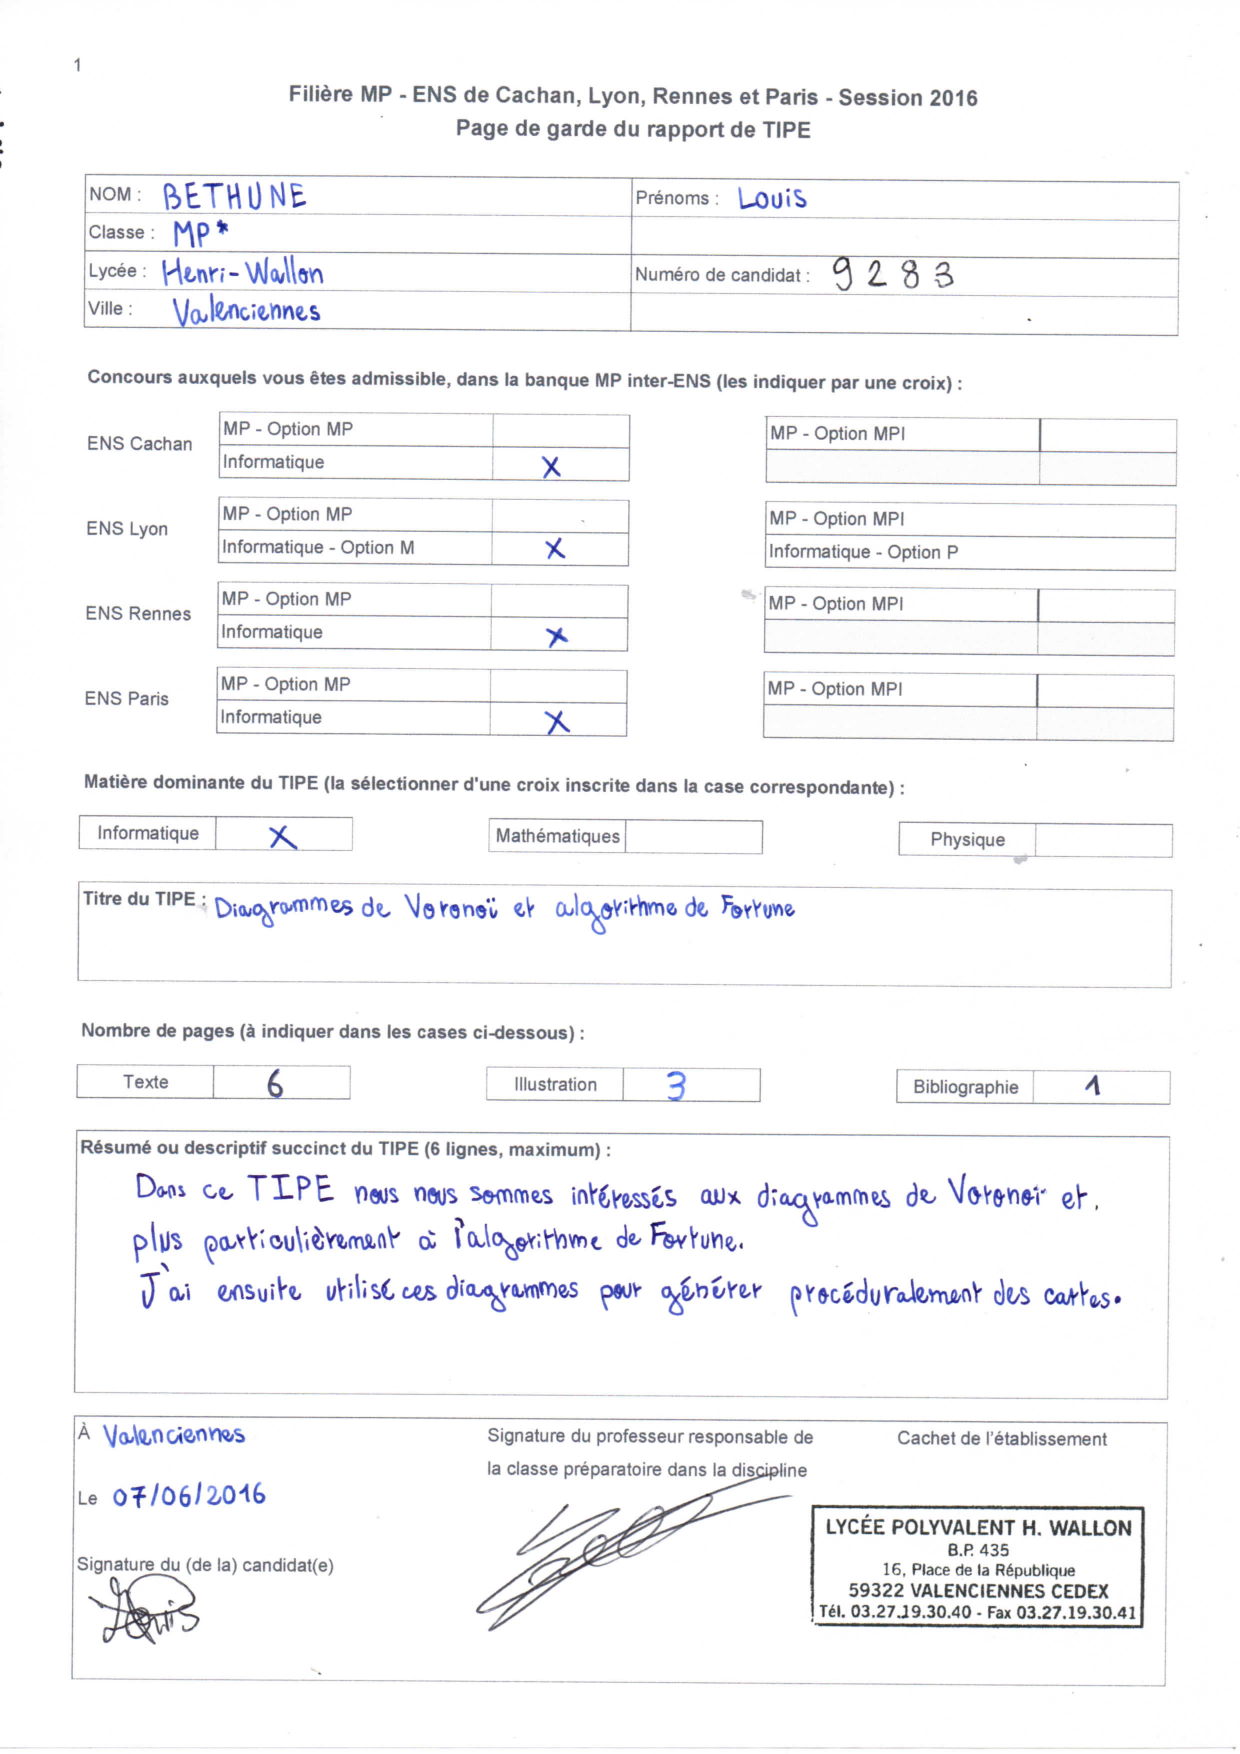
\includegraphics[scale=0.75]{enteteTIPE.pdf} 
\maketitle 
Notre objectif était d'étudier les diagrammes de Voronoï, et plus particulièrement l'algorithme de Fortune permettant de construire ces diagrammes de façon efficace. Cette partie est commune avec celle de mon binôme COIFFIER Guillaume.  
  
Ensuite, je me suis intéressé à la manière dont on peut utiliser les diagrammes de Voronoï pour effectuer de la génération procédurale de cartes polygonales. Pour ce faire j'applique une relaxation de Lloyd sur une distribution aléatoire de points dans le plan, afin de donner un aspect régulier au pavage. Puis j'utilise le bruit de Perlin pour affecter une hauteur à chacun des points du diagramme.  

\section{Diagrammes de Voronoï de points}  
Les diagrammes de Voronoï possèdent des applications dans de très nombreux domaines comme le machine learning, l'épidémiologie, la cristallographie, et comme solution intermédiaire à plusieurs problèmes de géométrie algorithmique.  
  
Soit $S$ un ensemble fini de points du plan $P$, nommés \textbf{sites}. La cellule de Voronoï d'un site $s$ est :  
$$C(s)=\{p\in P\;|\;d(s, p)\leq d(s', p)\;\forall s'\in S\}$$
C'est donc l'ensemble des points du plan qui sont plus proche du site $s$ que de tout autre site. Ainsi chaque cellule contient très exactement un site. Les cellules sont nécessairement convexes, car elles peuvent être définies comme une intersection finie de demi-plans.  

\begin{center}  
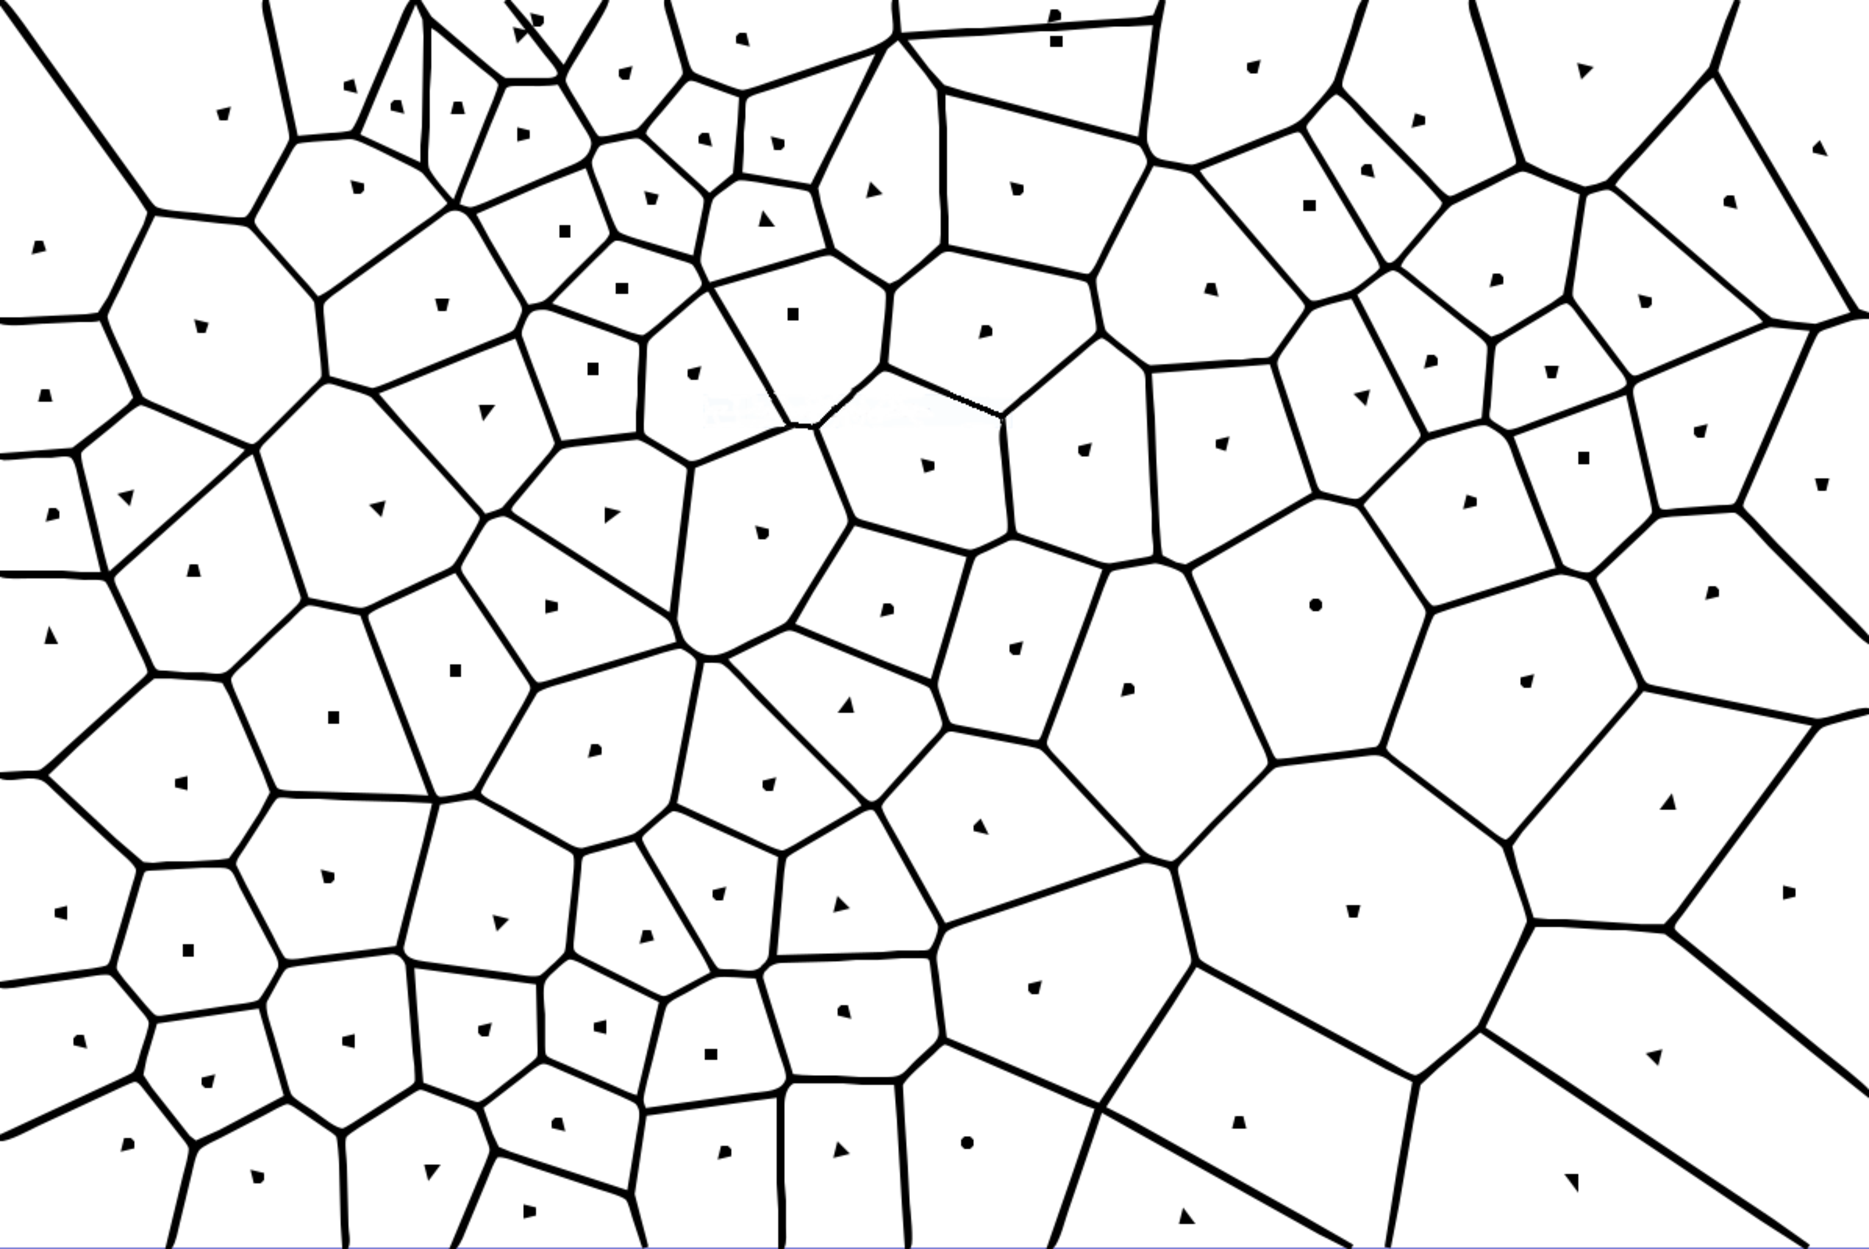
\includegraphics[scale=0.25]{PointsRelax.pdf}  
  
Diagramme de Voronoï d'une centaine de sites.
\end{center}
  
Deux cellules adjacentes sont séparées par une \textbf{arête} : elle est constituée des points équidistants de deux sites. En particulier toute arête est un morceau de la médiatrice du segment joignant les deux sites.  
  
Les arêtes (au minimum trois) s'intersectent en un \textbf{sommet} du diagramme, centre du cercle circonscrit à au moins trois sites, et dont l'intérieur du disque ne contient aucun autre site. Un tel disque est nommé \textbf{disque de Delaunay}.  
  
Le diagramme est défini comme la réunion de tout les sommets et toutes les arêtes : c'est un graphe, qui est planaire par construction. Les cellules pavent le plan.  
  
Il est possible de construire le diagramme en $\mathcal{O}(n^2)$ à l'aide d'un algorithme incrémental, qui actualise le diagramme courant à chaque ajout d'un nouveau site (algorithme de Green et Sibson, 1978). En 1975 Shamos et Hoey ont proposé un algorithme en $\mathcal{O}(n\log{n})$ qui s'appuie sur un diviser pour régner, qui fusionne deux sous-diagrammes à chaque étape de la récursion. Finalement, en 1987 Steve Fortune propose un autre algorithme de complexité $\mathcal{O}(n\log{n})$, réputé plus simple à implémenter que le précédent.  
\section{Algorithme de Fortune}  
L'algorithme de Fortune appartient à la famille des algorithmes dit \textbf{à ligne de balayage} : il s'appuie sur une droite virtuelle $\Delta$ qui balaye le plan dans le sens des ordonnées décroissantes. Le diagramme est construit au fur et à mesure.  
  
On a déjà vu que les points sur les arêtes sont équidistantes de deux sites. Comme l'ordonnée $y_{\Delta}$ de la ligne de balayage prend successivement la valeur de l'ordonnée des différents sites, il est naturel de considérer les points équidistants de la droite et des sites déjà rencontrés.  
Pour chaque site, l'ensemble des points vérifiant cette équation est une parabole ayant le site pour foyer. Chaque parabole définie une région de l'espace non bornée qui s'étend à l'infini \textit{derrière} la ligne de balayage. Ces régions peuvent se recouvrir. Les arcs de parabole qui ne sont inclus dans la région d'aucune autre parabole forment \textbf{le front parabolique}.  
  
\subsubsection{Point anguleux}
  
Deux arcs de paraboles du front s'intersectent en \textbf{un point anguleux}. La distance du point anguleux à chacun des deux sites est égale à la distance du point anguleux à la droite $\Delta$. Donc le point anguleux est à même distance des deux sites : il appartient donc à une arête du diagramme. Ainsi, au fur et à mesure que la ligne balaye, le front parabolique avance, et les points anguleux tracent les arêtes du diagramme.  
  
\begin{center}
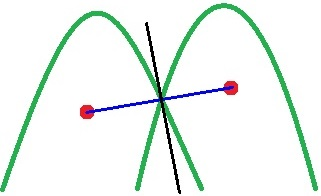
\includegraphics[scale=0.4]{PointAnguleux.jpg}  
  
L'arête (en noir) est la médiatrice du segment (en bleu) joignant les deux sites, elle est engendré par les paraboles (en vert). Les dimensions réelles ne sont pas respectées.  
\end{center}

\subsubsection{Évènement site : apparition d'arcs de parabole}
  
Chaque fois que la ligne de balayage rencontre un site (ce qu'on appellera désormais un \textbf{évènement site}), on crée une nouvelle parabole dégénérée (réduite à une demi-droite) qu'on insère dans le front parabolique. L'arc de parabole ainsi intersecté est coupé en deux morceaux, donnant naissance à deux \textbf{demi-arêtes}. On les nomme ainsi car chacune d'entre elle s'étend dans un sens différent, et leur "raccordement" donne l'arête finale. En général on ne connait pas immédiatement leurs autres extrémités. En particulier, on ne connait pas forcément les deux extrémités de l'arête du diagramme : on sait juste qu'elle existe et passe par ce point.  
  
\begin{center}
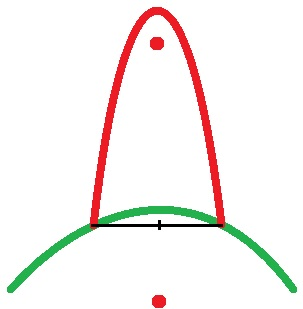
\includegraphics[scale=0.35]{EvenementSite.jpg}  
  
On observe ici les deux demi-arêtes (en noir) en cours de construction. La nouvelle parabole (en rouge) intersecte l'ancienne (en vert). Les dimensions réelles ne sont pas respectées.  
\end{center}
  
\subsubsection{Évènement cercle : disparition d'arcs de parabole}  
  
Certains arcs de parabole finissent par être réduit à un point, lorsque les deux arcs adjacents finissent par le recouvrir (cela arrive quand le site $s_m$ de l'arc disparu est plus éloigné de la ligne balayage que les sites $s_g$ et $s_d$ des deux autres arcs). À ce moment les deux points anguleux de part et d'autre sont confondus. Cela signifie donc que les deux arêtes s'intersectent en ce point, qui se trouve être un sommet du diagramme ! Comme il appartient aux deux arêtes, il est à même distance des trois sites, et donc il est bien le centre du cercle circonscrit aux trois sites, d'où la dénomination d'\textbf{évènement cercle}. On peut alors terminer les deux arêtes $a_g$ et $a_d$, et en créer une nouvelle, ayant pour direction celle de la médiatrice du segment $[s_g;s_d]$.  
  
\begin{center}
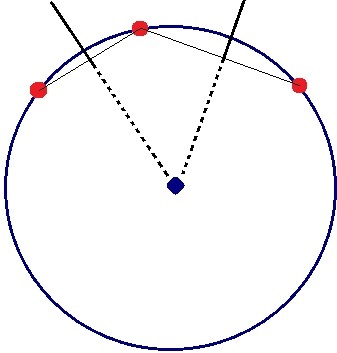
\includegraphics[scale=0.35]{EvenementCercle.jpg}  
  
On anticipe l'intersection des arêtes (en pointillés) sur un sommet du diagramme, centre du cercle circonscrit (en bleu). 
\end{center}
  
\section{Implémentation}  
L'algorithme décrit ci-dessus semble fonctionner comme si $\Delta$ balayait le plan de façon continue. Toutefois ce n'est pas nécessaire : il suffit de "sauter" aux endroits stratégiques pour obtenir les coordonnées des sommets du diagramme. On en déduit alors facilement les arêtes.  
  
\subsubsection{File à priorité et évènements}  
  
Pour cela on insère dans une file à priorité les évènements sites, triés selon l'ordonnée décroissante. Lors de la création des arêtes, on vérifie qu'elles n'intersectent pas une arête adjacente, auquel cas on crée un évènement cercle qu'on insère aussi dans la file. On remarque que la découverte d'un évènement site peut parfois invalider un évènement cercle déjà inséré. Dans ce cas là il faut penser à marquer les évènements cercles associés comme "périmés". Ils seront ignorés lorsqu'ils seront sortis de la file (principe du tas paresseux : on ne cherche pas à supprimer l'élément, on se contente de l'ignorer).  
  
\subsubsection{Gestion du front parabolique : utilisation d'un arbre binaire}  
  
La seconde difficulté consiste à insérer un nouvel arc parabolique dans le front. On pourrait utiliser une liste triée par abscisse (l'abscisse du site correspond à l'arc de parabole), mais les recherches et insertions se feraient en $\mathcal{O}(n)$ ce qui est prohibitif. Au lieu de ça on utilise un \textbf{arbre binaire} qui permet les mêmes opérations en $\mathcal{O}(\log{n})$ en moyenne, car c'est la profondeur moyenne d'un arbre binaire construit aléatoirement. Il est possible d'équilibrer cet arbre pour garantir une complexité logarithmique en toutes circonstances mais nous n'avons pas implémenté cette fonctionnalité.  
  
Contrairement à un arbre binaire de recherche, dans lequel les éléments sont stockés dans tous les nœuds de l'arbre, on choisit de stocker les arcs de paraboles exclusivement aux feuilles, qui se trouvent être ordonnées par abscisses croissantes. On sait que les arêtes se situent toujours entre deux feuilles. Or on peut mettre en bijection les nœuds (non feuillus) de l'arbre avec une paire de deux feuilles consécutives ! Chaque nœud non feuillu enjambe exactement deux feuilles consécutives, on peut donc y stocker l'arête séparant les deux arcs de parabole.  
  
\begin{center}
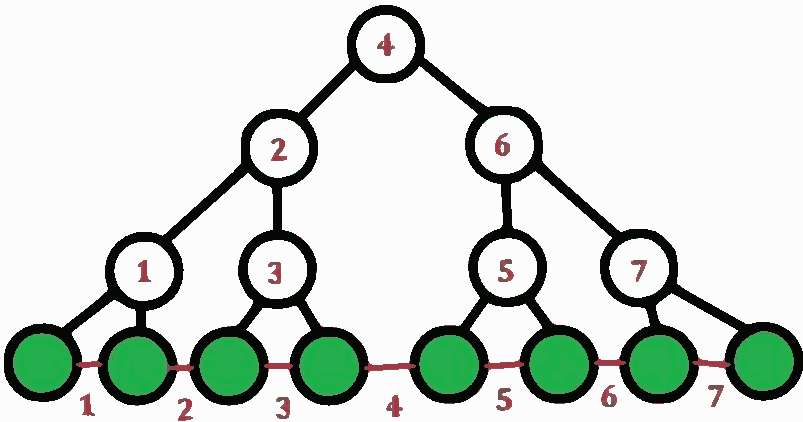
\includegraphics[scale=0.4]{ArbreBinaire-vect.pdf}  
  
Les positions des arêtes sont numérotés en rouge. On observe qu'il y a bien bijection entre le nœud et l'intervalle.  
\end{center}
  
Depuis un arc on peut donc accéder à l'arête adjacente, et vice-versa, en $\mathcal{O}(\log{n})$ en moyenne.    
  
\subsubsection{Pseudo-code}  
\begin{itemize}
\item Ensemble de sites $\mathcal{S}$
\item File à priorité $\mathcal{F}$
\item Tableau d'arêtes $\mathcal{E}$
\item Tableau de sommets $\mathcal{V}$
\item Arbre du front parabolique $\mathcal{A}$
\end{itemize}

\begin{tabbing}
\hspace{0.5cm} \= \hspace{0.5cm} \= \hspace{0.5cm} \= \hspace{0.5cm} \= \kill
\textsc{Procédure Fortune($\mathcal{S}$) :} \\  
\> Insérer tous les évènements sites de $\mathcal{S}$ dans $\mathcal{F}$ \\
\> Tant que $\mathcal{F}$ est non vide \\  
\> \> Extraire de $\mathcal{F}$ un évènement $\mathsf{e}$ \\ 
\> \> Si $\mathsf{e}$ est un évènement site \\
\> \> \> Créer $P_m$ la parabole de site $\mathsf{e.site}$\\
\> \> \> Trouver $P$ la parabole dans $\mathcal{A}$ intersectée par $P_m$, de site $\mathsf{s}$, et soit $\mathsf{v}$ le point d'intersection \\
\> \> \> Marquer l'évènement cercle associé à $P$ comme périmé \\  
\> \> \> Créer deux demi-arêtes $A_g$ et $A_d$ d'extrémité $\mathsf{v}$, entre $\mathsf{e}.\mathsf{site}$ et $\mathsf{s}$, et en ajouter une dans $\mathcal{E}$ \\
\> \> \> Soit $P_g$ et $P_d$ deux paraboles de site $\mathsf{v}$ \\  
\> \> \> Remplacer $P$ par la séquence $(P_g, A_g, P_m, A_d, P_d)$ \\
\> \> \> \textsc{TesterÉvènementCercle}($P_g$) \\
\> \> \> \textsc{TesterÉvènementCercle}($P_d$) \\
\> \> Si $\mathsf{e}$ est un évènement cercle non périmé \\
\> \> \> Soit $P$ la parabole de $\mathcal{A}$ associée à $\mathsf{e}$ \\
\> \> \> Soit $P_g$ et $P_d$ les paraboles de $\mathcal{A}$ voisines de $P$ \\
\> \> \> Marquer les évènements cercles associés à $P_g$ et $P_d$ comme périmés \\
\> \> \> Soit $A_g$ et $A_d$ les arêtes de $\mathcal{E}$ voisines de $P$ \\
\> \> \> Soit $\mathsf{v}$ le point d'intersection de $A_g$ et $A_d$, l'ajouter à $\mathcal{V}$ \\  
\> \> \> Terminer les arêtes $A_g$ et $A_d$ avec $\mathsf{v}$ \\
\> \> \> Créer une nouvelle arête $A_m$ partant de $\mathsf{v}$ et l'ajouter à $\mathcal{E}$\\  
\> \> \> Remplacer la séquence $(A_g, P, A_d)$ par $A_m$ \\  
\> \> \> \textsc{TesterÉvènementCercle}($P_g$) \\
\> \> \> \textsc{TesterÉvènementCercle}($P_d$) \\
\> Pour chaque arête $\mathsf{e}$ dans $\mathcal{E}$ \\
\> \> Si $\mathsf{e}$ est une demi-arête \\  
\> \> \> Raccorder $\mathsf{e}$ et $\mathsf{e.voisin}$ \\
\textsc{Fin de la procédure}
\end{tabbing} 
\begin{tabbing}
\hspace{0.5cm} \= \hspace{0.5cm} \= \hspace{0.5cm} \= \hspace{0.5cm} \= \kill
\textsc{Procédure TesterÉvènementCercle($P$) :} \\
\> Soit $P_g$ et $P_d$ les paraboles de $\mathcal{A}$ voisines de $P$ \\
\> Soit $A_g$ et $A_d$ les arêtes de $\mathcal{E}$ voisines de $P$ \\
\> Si $P_g$, $P_d$, $A_g$ ou $A_d$ n'existe pas \\ 
\> \> \textsc{Sortir} \\
\> Soit $\mathsf{v}$ le point d'intersection des deux arêtes \\
\> Soit $\mathsf{d}$ la distance de $\mathsf{v}$ au site de $P$ \\
\> Si $\mathsf{v.y-d}$ est avant la ligne de balayage \\
\> \> \textsc{Sortir} \\
\> Ajouter dans $\mathcal{F}$ un évènement cercle au point de coordonnées $\mathsf{(v.x, v.y-d)}$ \\  
\> Associer cet évènement à $P$ \\
\textsc{Fin de la procédure}
\end{tabbing}  
\subsubsection{Analyse et résultats}  
Notre implémentation demeure un $\mathcal{O}(n^2)$ en pire des cas, néanmoins elle se comporte comme un $\mathcal{O}(n\log{n})$ en moyenne, sur une distribution aléatoire de points (ce que l'on peut vérifier sur les \textbf{figures 1 et 2}).   
  
La manière dont les évènements cercles sont traités ne permet de gérer que le cas de trois points cocycliques. Lorsque que plus de deux arêtes sont concourantes (par exemple lorsque les sites sont aux coins d'un carré) l'algorithme renvoie un résultat incohérent. Heureusement, les chances qu'un tel évènement survienne sont faibles sur une distribution aléatoire de points.  
  
Sur une distribution réelle de points, on pourra par exemple limiter cet effet en perturbant les coordonnées de chaque site d'un $\epsilon$. Cela suffira à rendre les points non cocycliques (avec une forte probabilité) tout en conservant l'allure générale du diagramme.  
  
\section{Génération procédurale de cartes}  
  
La génération procédurale est la création de contenu numérique à grande échelle, de façon automatisée et aléatoire. Elle est très utilisée dans le domaine du jeu vidéo, et plus particulièrement celui de la génération de \textit{maps} (comme \textit{Age of empire}, \textit{Civilisation}, \textit{Minecraft}), ce qui permet de proposer à l'utilisateur du contenu très diversifié en quantité presque illimitée.  
  
Néanmoins l'utilisation d'un aléatoire non contrôlé conduit suivant à des résultats aberrants. On préférera donc un processus \textbf{semi-aléatoire}, produisant des résultats localement chaotiques mais globalement cohérents.  

\subsubsection{Cartes polygonales}
  
Il peut-être intéressant de découper la carte en différentes \textbf{régions}. C'est la première étape d'un traitement plus fin qui consistera ensuite à générer le contenu de ces régions (altitude, végétation, village, rivières, forêts, montagnes, ressources... ). Le moyen le plus couramment employé est l'utilisation d'une grille bidimensionnelle régulière, où toutes les régions sont de forme carrée et de mêmes dimensions. On peut également trouver des pavages hexagonaux du plan. Cependant la régularité trop importante de ces pavages peut donner un aspect irréaliste à la carte.  
  
En revanche un pavage formé de différents polygones, espacés de façon régulière mais non constante donne un aspect plus naturel et plus chaotique, conformément à l'intuition que l'on se fait d'un terrain.  
  
Ainsi les diagrammes de Voronoï sont tout indiqués : on tire au hasard des points dans le plan, on en calcule le diagramme, et les cellules de notre diagrammes pavent le plan. Plus les points seront nombreux et plus les cellules seront petites, et donc plus le maillage sera fin.  
  
\subsubsection{Relaxation de Lloyd}
Une distribution purement aléatoire contient parfois des zones avec beaucoup de sites (très proches les uns des autres) et d'autres zones où ils sont plus rares (et les cellules plus grandes). Pour éviter ça on peut appliquer une \textbf{relaxation de Lloyd}. Cet algorithme calcule le diagramme de Voronoï d'un ensemble de sites, puis calcule le barycentre de chacune des cellules. Il y a donc autant de barycentres que de sites, et on peut calculer le diagramme de Voronoï de ces barycentres. Cette procédure peut être appliquée autant de fois que souhaité (voir \textbf{figures 3, 4 et 5}). Généralement une seule fois suffit.  
  
\subsubsection{Height map et bruit de Perlin}  
Il est nécessaire d'affecter une altitude à chaque sommet du diagramme. Ensuite, on définie la hauteur de chaque site comme la moyenne des hauteurs des sommets de sa cellule. Le terrain est alors composé de plein de petits triangles à l'allure caractéristique (voir \textbf{figure 6}).  
  
Pour déterminer la hauteur de chaque sommet on utilise le \textbf{bruit de Perlin}, mis au point par Ken Perlin en 1985. C'est un algorithme produisant un bruit de gradient : il est donc parfaitement adapté à la génération de gradients d'altitude.  
\newpage
\begin{tabbing}
\hspace{0.5cm} \= \hspace{0.5cm} \= \hspace{0.5cm} \= \hspace{0.5cm} \= \kill
\textsc{Procédure PerlinNoise}(\textbf{Tableau de sommets} $\mathcal{V}$, \textbf{Fréquence} $\mathsf{f}$, \textbf{Amplitude} $\mathsf{a}$, \textbf{Fonction} $\mathsf{interpoler}$) : \\
\> Soit $\mathcal{G}$ une grille bidimensionnelle, de largeur $\mathsf{f}$, à cases carrées, et recouvrant une partie du plan contenant $\mathcal{V}$ \\
\> Pour chaque sommet $\mathsf{c}$ de $\mathcal{G}$ \\
\> \> Calculer la position $\mathsf{c.p}$ \\
\> \> Affecter un vecteur unitaire de direction aléatoire à $\overrightarrow{\mathsf{c.g}}$ \\
\> Pour chaque sommet $\mathsf{v}$ de $\mathcal{V}$ \\
\> \> Déterminer la case $\mathcal{C}$ de $\mathcal{G}$ à laquelle appartient $\mathsf{v}$ \\
\> \> \textbf{Tableau de flottants} $\mathcal{W}$ de taille $2\times 2$ \\
\> \> Pour chaque coin $\mathsf{c}$ de $\mathcal{C}$ \\
\> \> \> Calculer $\overrightarrow{\mathsf{c.g}}\cdot \frac{\overrightarrow{\mathsf{c.p}}-\overrightarrow{\mathsf{v.p}}}{\|\overrightarrow{\mathsf{c.p - v.p}\|}}$ et l'ajouter à $\mathcal{W}$ \\
\> \> $\mathsf{y_1} \longleftarrow \mathsf{interpoler}(\mathcal{W}\mathsf{[Haut][Gauche]}, \mathcal{W}\mathsf{[Haut][Droite]})$ \\
\> \> $\mathsf{y_2} \longleftarrow \mathsf{interpoler}(\mathcal{W}\mathsf{[Bas][Gauche]}, \mathcal{W}\mathsf{[Bas][Droite]})$ \\
\> \> $\mathsf{z_0} \longleftarrow \mathsf{interpoler}(\mathsf{y_1}, \mathsf{y_2})$ \\
\> \> $\mathsf{v.z \longleftarrow v.z+\mathsf{z_0\times a}}$ \\
\textsc{Fin de la procédure}
\end{tabbing}
Cet algorithme peut être appliqué autant de fois que nécessaire, avec des fréquences chaque fois plus grandes et des amplitudes chaque fois plus basses. Ainsi les basses fréquences dessinent "les grandes lignes" du relief (montagnes, vallées... ) et les hautes fréquences permettent d'en moduler la granularité (voir \textbf{figure 8}). On utilisera le terme "d'octave" pour chacune des applications du bruit liée à une fréquence particulière.  
  
La fonction d'interpolation renvoie $a+f(t)(b-a)$ avec $a$ et $b$ les valeurs que l'on interpole, et $t \in [0,1]$ un paramètre réel qui ne dépend que de la projection du sommet sur le segment joignant les coordonnées de $a$ et $b$.  
  
La fonction $f$ peut-être choisie librement, du moment qu'elle est croissante sur $[0,1]$ à valeurs dans $[0,1]$, avec $f(0)=0$ et $f(1)=1$. On peut par exemple prendre $Id_{\mathbb{R}}$ ce qui donnera une interpolation linéaire, ou quelque chose de plus compliqué (un polynôme de degré supérieur, une fonction sinusoïdale...).
\subsubsection{Îles}  
Le bruit de Perlin donne des résultats assez satisfaisants mais ne permet pas de contrôler finement les formes du territoire (choisir la position des montagnes ou des lacs). On aimerait par exemple pouvoir générer des îles (zone centrale élevée, entourée d'eau).   
  
Pour ce faire on introduit un terme correctif : on calcule la distance de chaque sommet au centre de l'image (ce centre pouvant être défini de façon arbitraire par translation de l'origine). Cette distance est ensuite normalisée (divisée par sa valeur maximum) pour être ramenée entre $0$ et $1$, appelons la $d_0$. On multiplie alors les hauteurs $\mathsf{v.z}$ par $e^{-ad_0}+b$. Les paramètres $a$ et $b$ peuvent être réglés par essais-erreurs selon le résultat souhaité.  
  
Cette formule tend à élever le relief proche du centre, et à abaisser celui qui s'en éloigne. Il en résulte l'apparition d'une "île" près du centre.    
\subsubsection{Couleurs}  
Une correspondance a été établie manuellement entre la hauteur et la couleur d'une région. Ainsi en dessous de certains seuils on trouvera la mer, la plage, la forêt, la montagne, la neige... certains intervalles de hauteur sont associés à un dégradé de couleur (eau et forêt) pour que le résultat soit plus agréable au regard. Ici comme dans la partie précédente, les critères de choix sont moins d'ordre technique que esthétique.  

\newpage
\section{Bibliographie}  
\begin{itemize}
\item D. Beauquier, J. Berstel, Ph. Chrétienne, \textit{Éléments d'algorithmique}, 2005  
  
\item Vincent Pilaud, \textit{Sur le diagramme de Voronoi et la triangulation de Delaunay d’un ensemble de points dans un revêtement du plan euclidien}, 2006  

\item Franck Hétroy, \textit{Un petit peu de géométrie algorithmique}, cours de Grenoble INP Ensimag
  
\item Ivan Kuckir, \textit{Fortune’s algorithm and implementation},  
  
\url{http://blog.ivank.net/fortunes-algorithm-and-implementation.html}      
  
\item Wikipédia, \textit{Fortune's algorithm}, 

\url{https://en.wikipedia.org/wiki/Fortune's_algorithm}    
  
\item Matt Brubeck, \textit{Fortune's Algorithm in C++},  
  
\url{https://www.cs.hmc.edu/~mbrubeck/voronoi.html}  

\item Red Blob Games, \textit{Polygonal Map Generation for Games},   
  
\url{http://www-cs-students.stanford.edu/~amitp/game-programming/polygon-map-generation/}  
  
\item Développez, \textit{Génération de terrain par l'algorithme de Perlin},  
  
\url{http://khayyam.developpez.com/articles/algo/perlin/}  
  
\item Adrian's soap box, \textit{Understanding Perlin Noise},  
  
\url{http://flafla2.github.io/2014/08/09/perlinnoise.html}
\end{itemize}
\newpage
\section{Figures}  
\begin{center}
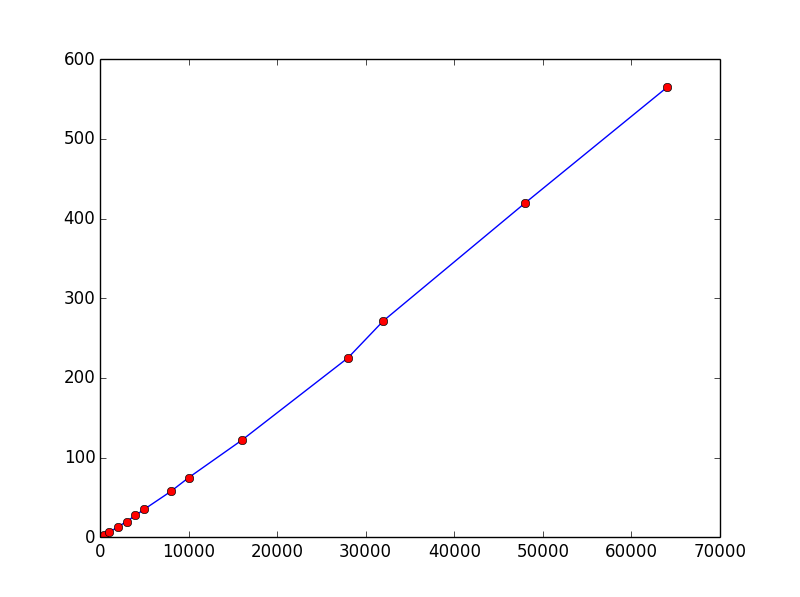
\includegraphics[scale=0.4]{PerformancesMilisecondes.png} 
  
\textbf{Figure 1}: nombre de sites en abscisse, et temps de calcul en ordonnée (en millisecondes) sur un Intel(R) Core(TM) i3-4010U CPU cadencé à 1.7GHz. Les temps pour les petits ensembles de points (inférieurs à 10 000) ont été moyennés sur plusieurs dizaines d'exécutions.  
  
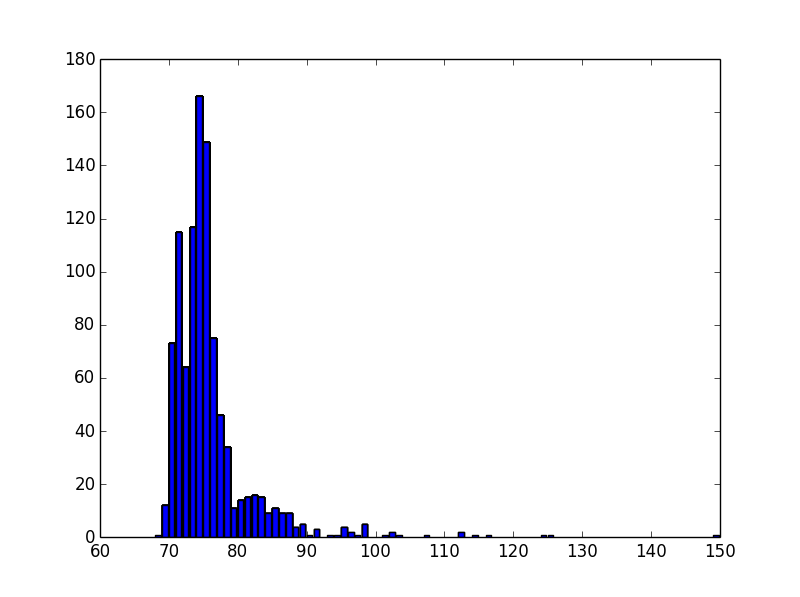
\includegraphics[scale=0.4]{PerformancesGaussienne.png}  
  
\textbf{Figure 2}: répartition des temps de calcul pour 1000 exécutions d'un ensemble de 10 000 points générés aléatoirement. En abscisse le temps de calcul (en millisecondes) et en ordonnée les effectifs. La courbe a l'allure d'une distribution à "queue épaisse". La plupart des temps se concentrent autour de la moyenne mais certains sont jusqu'à deux fois plus long.  
\newpage
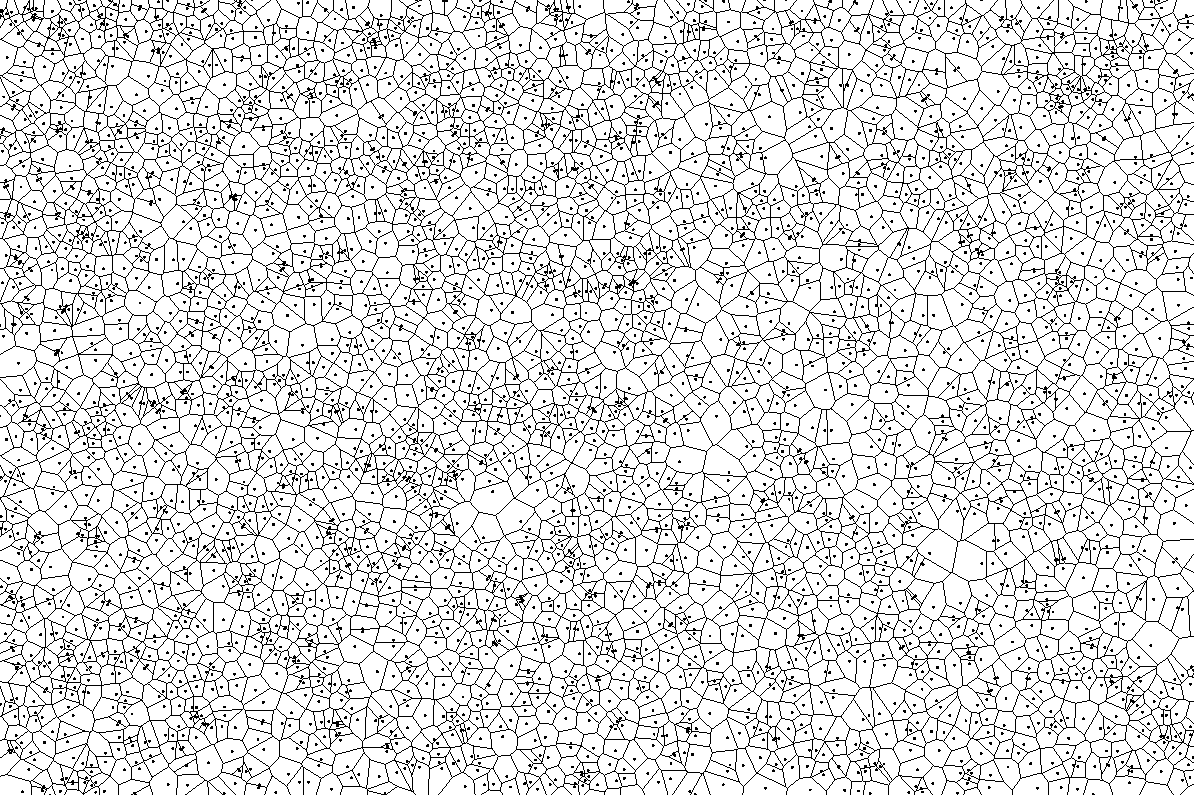
\includegraphics[scale=0.2]{Lloyd0.png}
  
\textbf{Figure 3}: diagramme de Voronoï d'un ensemble de 4000 points tirés au hasard.  
  
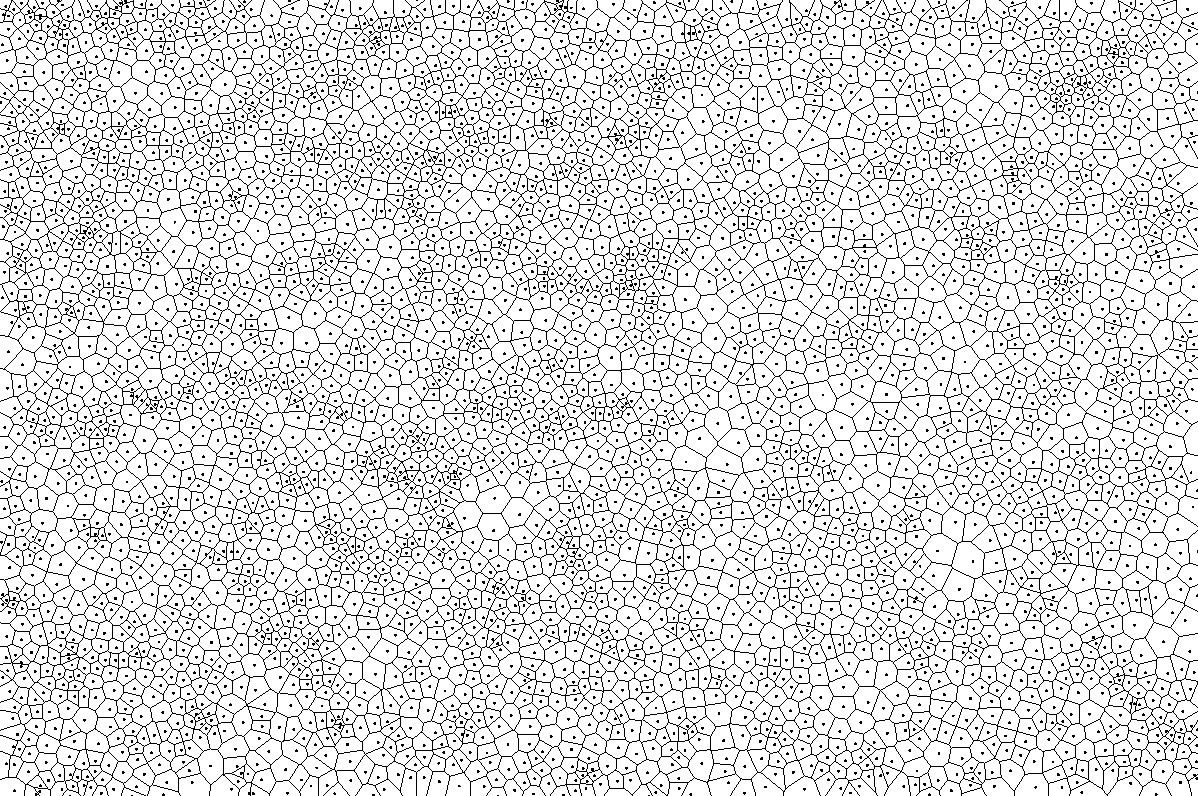
\includegraphics[scale=0.2]{Lloyd1.png}
  
\textbf{Figure 4}: même ensemble de points que \textbf{Figure 3}, après une itération de la relaxation de Lloyd.  
  
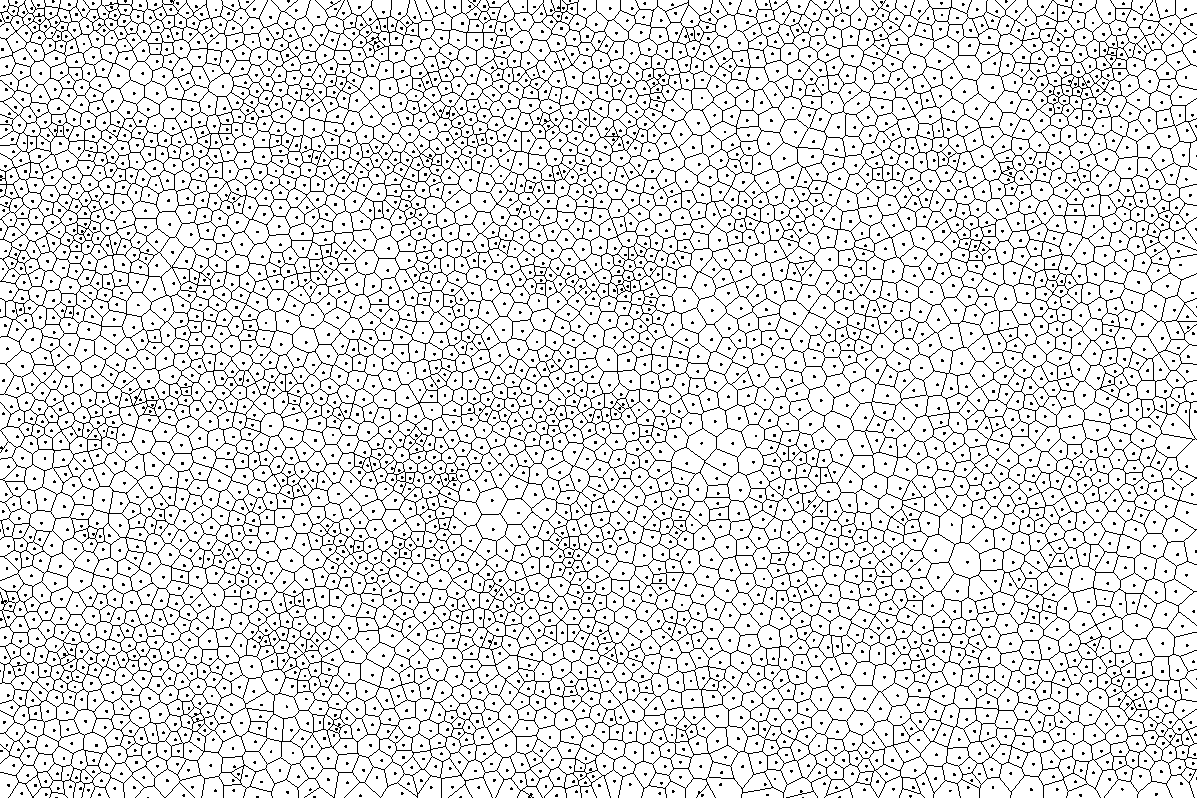
\includegraphics[scale=0.2]{Lloyd2.png}
  
\textbf{Figure 5}: même ensemble de points que \textbf{Figure 3}, après deux itérations de la relaxation de Lloyd.  

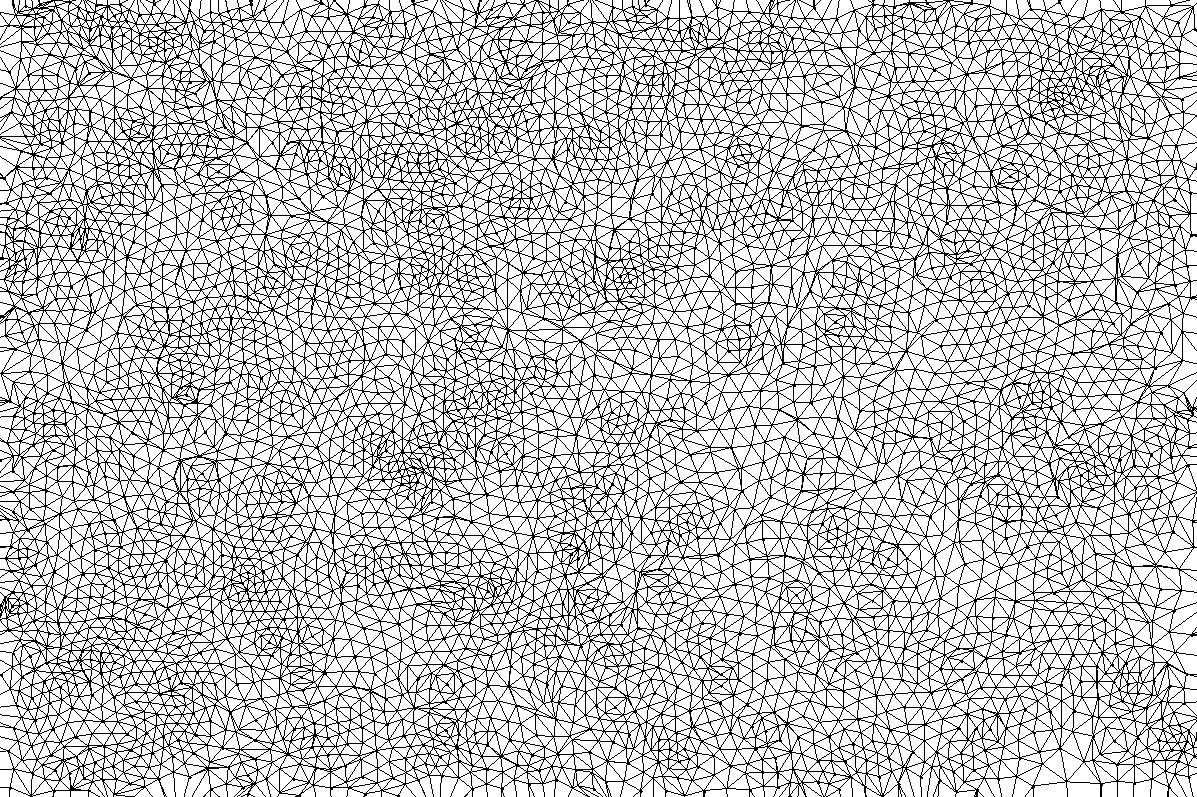
\includegraphics[scale=0.2]{AretesPoutres2000.png}
  
\textbf{Figure 6}: diagramme de Voronoï de 2000 points, avec en plus les rayons joignant chaque site aux sommets de sa cellule. Ne pas confondre avec la triangulation de Delaunay (figure 7).  
  
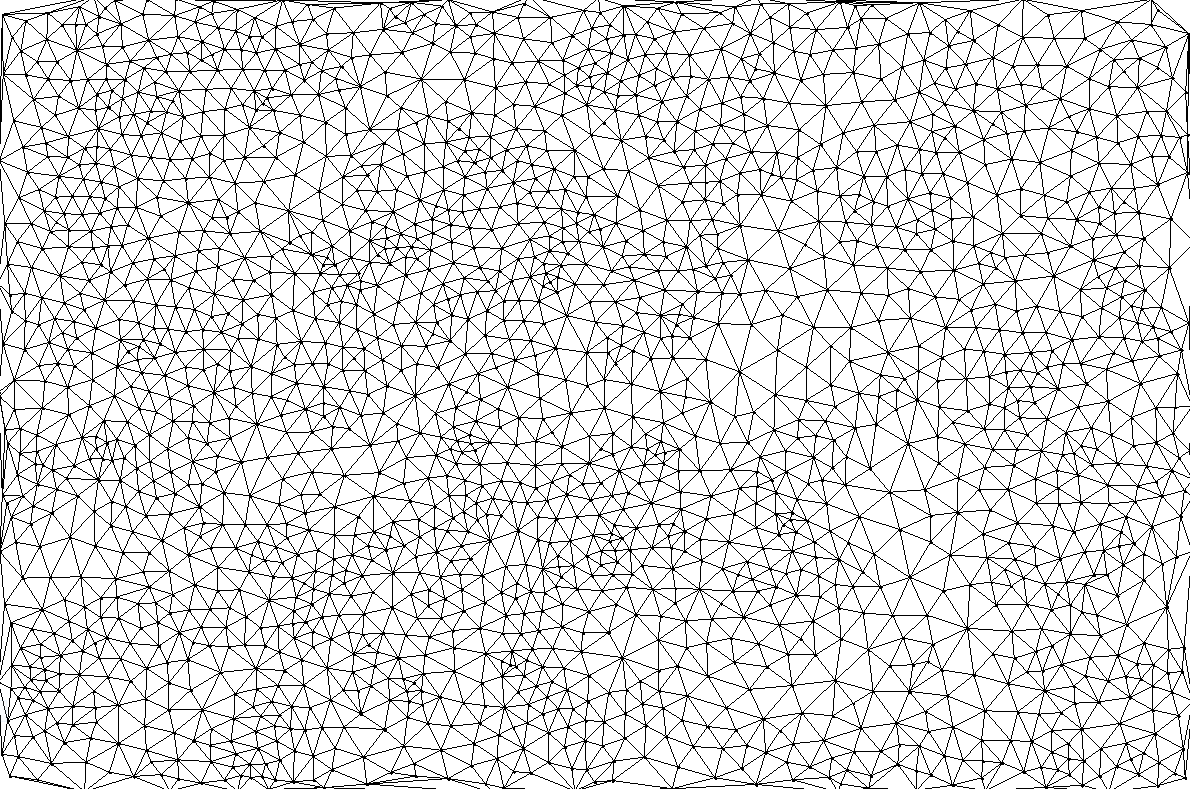
\includegraphics[scale=0.2]{DelaunayTriangulation2000.png}
  
\textbf{Figure 7}: triangulation de Delaunay de 2000 points, graphe dual du diagramme de Voronoï (relaxé deux fois).  
  
\bigbreak
\bigbreak
  
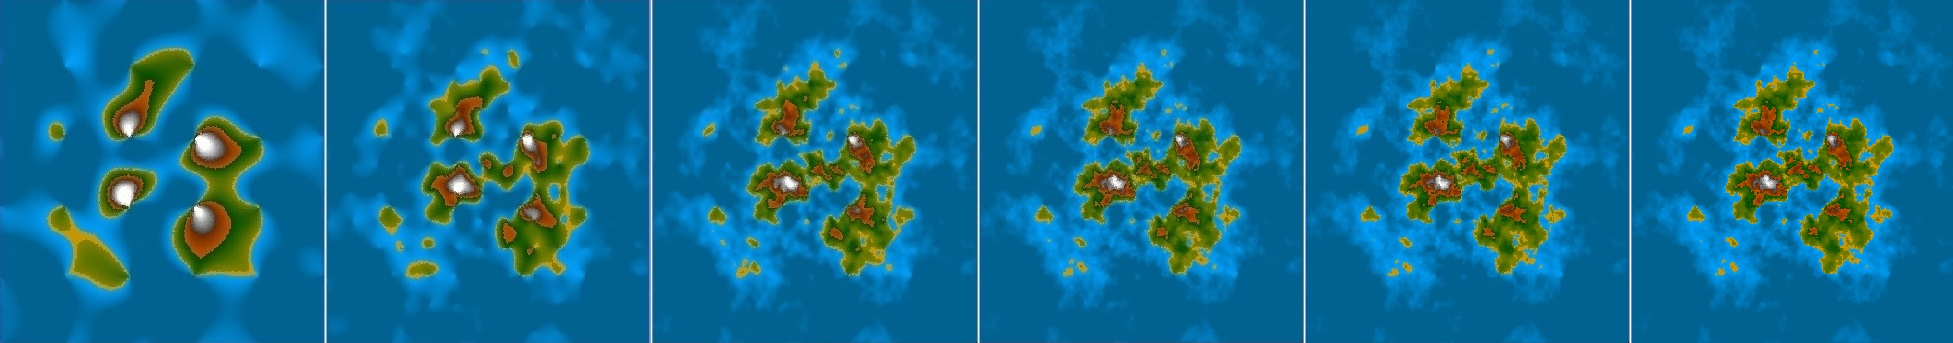
\includegraphics[scale=0.35]{Octaves.jpg}
  
\textbf{Figure 8}: six octaves du bruit de Perlin sur la même carte (64 000 polygones).  
  
\bigbreak
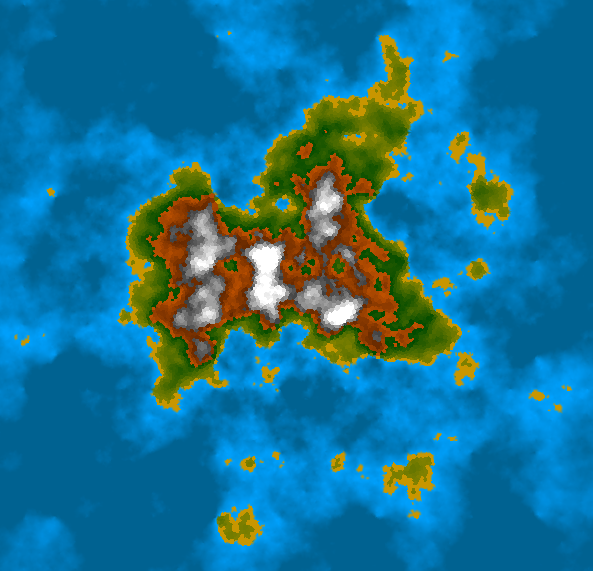
\includegraphics[scale=0.4]{Ile1.PNG}
  
\textbf{Figure 9}: autre île (64 000 polygones).  
  
\bigbreak
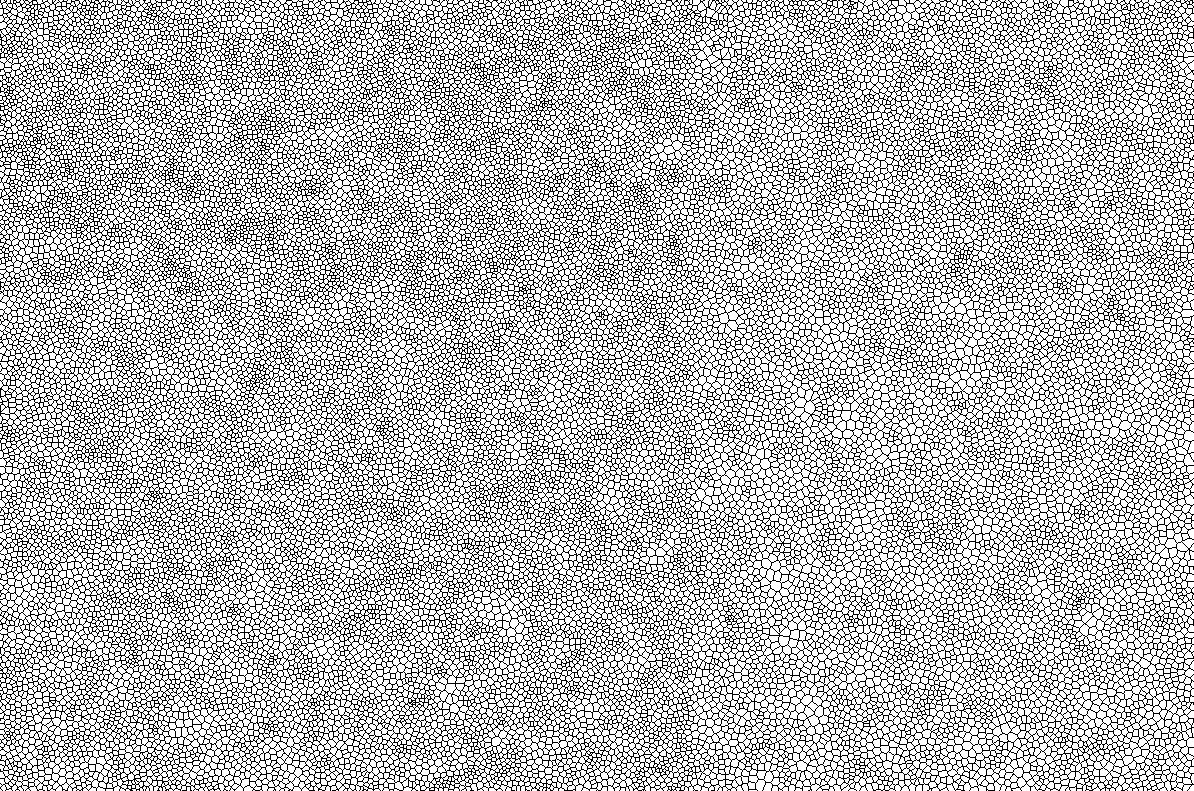
\includegraphics[scale=0.3]{Voronoi32000.PNG}
  
\textbf{Figure 9}: diagramme de Voronoï de 32 000 sites (non affichés) après deux relaxations.  
\end{center}  
\newpage
\section{Code source}  
On trouvera l'algorithme de Fortune dans \textbf{FortuneProcedure.h} et \textbf{FortuneProcedure.cpp}, le bruit de Perlin et la génération d'îles dans \textbf{PerlinNoise.h} et \textbf{PerlinNoise.cpp}. \textbf{VoronoiDiagram.h} et \textbf{VoronoiDiagram.cpp} définissent la structure de graphe et la relaxation de Lloyd, ainsi que d'autres utilitaires. \textbf{GeometricUtility.h} et \textbf{GeometricUtility.cpp} contiennent quelques fonctions pratiques. \textbf{VoronoiDiagram.cuh} et \textbf{VoronoiDiagram.cu} implémente la génération d'un diagramme de Voronoï massivement parallélisé sur carte graphique avec la technologie CUDA. 
\subsubsection{main.cpp}
\lstinputlisting[language=c++,breaklines = true,numbers=left,tabsize=2]{../SourceFiles/main.cpp}
\newpage
\subsubsection{VoronoiDiagram.h}
\lstinputlisting[language=c++,breaklines = true,numbers=left,tabsize=2]{../SourceFiles/VoronoiDiagram.h}
\newpage
\subsubsection{VoronoiDiagram.cpp}
\lstinputlisting[language=c++,breaklines = true,numbers=left,tabsize=2]{../SourceFiles/VoronoiDiagram.cpp}
\newpage
\subsubsection{Fortune.h}
\lstinputlisting[language=c++,breaklines = true,numbers=left,tabsize=2]{../SourceFiles/FortuneProcedure.h}
\subsubsection{Fortune.cpp}
\lstinputlisting[language=c++,breaklines = true,numbers=left,tabsize=2]{../SourceFiles/FortuneProcedure.cpp}
\newpage
\subsubsection{GeometricUtility.h}
\lstinputlisting[language=c++,breaklines = true,numbers=left,tabsize=2]{../SourceFiles/GeometricUtility.h}
\subsubsection{GeometricUtility.cpp}
\lstinputlisting[language=c++,breaklines = true,numbers=left,tabsize=2]{../SourceFiles/GeometricUtility.cpp}
\newpage
\subsubsection{PerlinNoise.h}
\lstinputlisting[language=c++,breaklines = true,numbers=left,tabsize=2]{../SourceFiles/PerlinNoise.h}
\subsubsection{PerlinNoise.cpp}
\lstinputlisting[language=c++,breaklines = true,numbers=left,tabsize=2]{../SourceFiles/PerlinNoise.cpp}
\newpage
\subsubsection{PerlinNoise.cuh}
\lstinputlisting[language=c++,breaklines = true,numbers=left,tabsize=2]{../SourceFiles/PerlinNoise.cuh}
\subsubsection{PerlinNoise.cu}
\lstinputlisting[language=c++,breaklines = true,numbers=left,tabsize=2]{../SourceFiles/PerlinNoise.cu}
\newpage
\subsubsection{VoronoiDiagram.cuh}
\lstinputlisting[language=c++,breaklines = true,numbers=left,tabsize=2]{../SourceFiles/VoronoiDiagram.cuh}
\subsubsection{VoronoiDiagram.cu}
\lstinputlisting[language=c++,breaklines = true,numbers=left,tabsize=2]{../SourceFiles/VoronoiDiagram.cu}
\end{document}
